% Created 2021-06-16 Mi 06:19
% Intended LaTeX compiler: pdflatex
\documentclass[11pt]{article}
\usepackage[utf8]{inputenc}
\usepackage[T1]{fontenc}
\usepackage{graphicx}
\usepackage{grffile}
\usepackage{longtable}
\usepackage{wrapfig}
\usepackage{rotating}
\usepackage[normalem]{ulem}
\usepackage{amsmath}
\usepackage{textcomp}
\usepackage{amssymb}
\usepackage{capt-of}
\usepackage{hyperref}
\usepackage{caption}
\usepackage{subcaption}
\usepackage[backend=bibtex]{biblatex}
\bibliography{refs}
\author{Laurent Lejeune}
\date{\today}
\title{BlueOrtho: Assignment}
\hypersetup{
 pdfauthor={Laurent Lejeune},
 pdftitle={BlueOrtho: Assignment},
 pdfkeywords={},
 pdfsubject={},
 pdfcreator={Emacs 27.1 (Org mode 9.5)}, 
 pdflang={English}}
\begin{document}

\maketitle

\section{Context and Goal}
\label{sec:org82fb568}

In the context of shoulder surgery, we aim at devising an algorithm
that segments scapulae on CT scans.
The provided dataset consists of synthetic and simplified shapes that
represent a humerus and a scapula.
Furthermore, the images are small (\(32\times32\)), and contain an important amount of noise.

A preview is shown on Fig. \ref{fig:input_prev}

\begin{figure}[htbp]
\centering
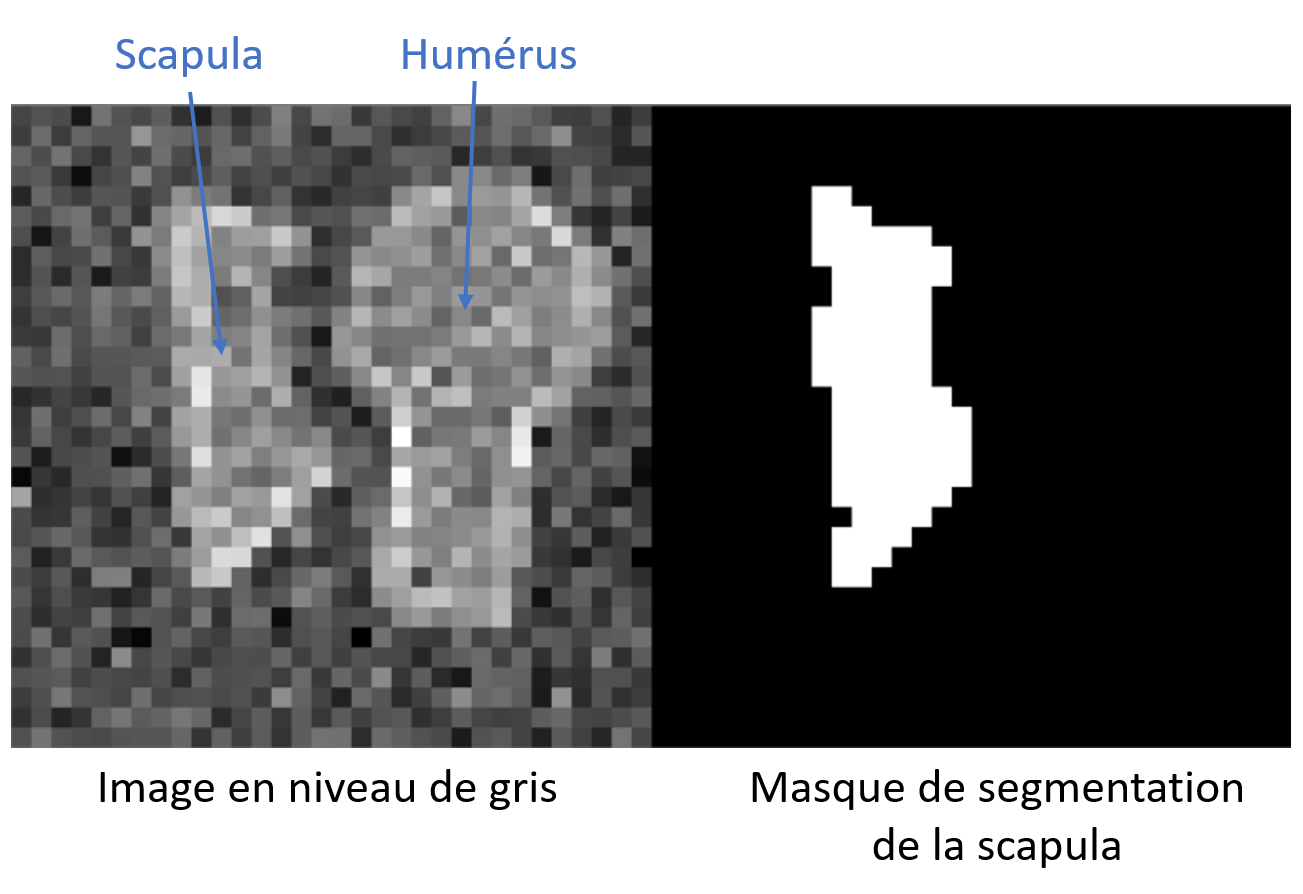
\includegraphics[width=.9\linewidth]{./input_prev.png}
\caption{\label{fig:input_prev}Example image with its ground truth mask taken from the provided synthetic dataset.}
\end{figure}

\section{Method}
\label{sec:orgcc1a353}

For this exercise, we choose to use a Convolutional Neural Network (CNN) that takes as input
a grayscale image, and outputs a probability map of same shape, where pixels with values close to \(1\) must belong to the scapulae, while others must be close to \(0\).

While many CNN solutions already exist, e.g. U-Net \cite{ronneberger15}, DeepLab \cite{chen18}, the specificity of this exercise justifies that
we devise a simpler and shallower architecture, which will relieve both training and inference
time.

In the next section, we present our architecture and justify the dimensions of
its components.
In a second section, we focus on the training objective and suggest two alternatives: Binary cross-entropy and Dice loss.

\subsection{Architecture}
\label{sec:org4c83501}

Our model follows the encoder-decoder principle, where the encoder
takes an input image to provide
features, while the decoder generates a probability map from the latter features.

\subsubsection{Encoder}
\label{sec:orgfa25f78}

For the encoder, we take inspiration from ShuffleNet-v2 \cite{ma18}.
In a nutshell, the latter leverages depth-wise convolutions and
inverted residual blocks to reduce the memory requirement.
This makes our model much faster in a low-resource scenario.

In contrast with the original ShuffleNet-v2, we reduce the number
of stages to \(3\) stages (instead of \(5\)), where each stages contains a
residual block.
The last bottleneck layer of our encoder thus provides feature tensor of shape \(8\times8\times32\).

\subsubsection{Decoder}
\label{sec:org341037e}

Our decoder follows the approach of \cite{chen18}, where features at the bottleneck
are expanded by a serie of ``Atrous'' convolutional layers with varying dilation rate, thereby forming an ``Atrous Spatial Pyramid Pooling'' (ASPP) block.
Also, low-level features, extracted at the earliest stage of the encoder are concatenated
to the output of the ASPP block.
In contrast to \cite{chen18}, we only use \(2\) Atrous layers (instead of \(4\)) with dilation
rates \(2\) and \(4\).

We give an illustration of our architecture on Fig. \ref{fig:deeplabv3p}.

\begin{figure}[htbp]
\centering
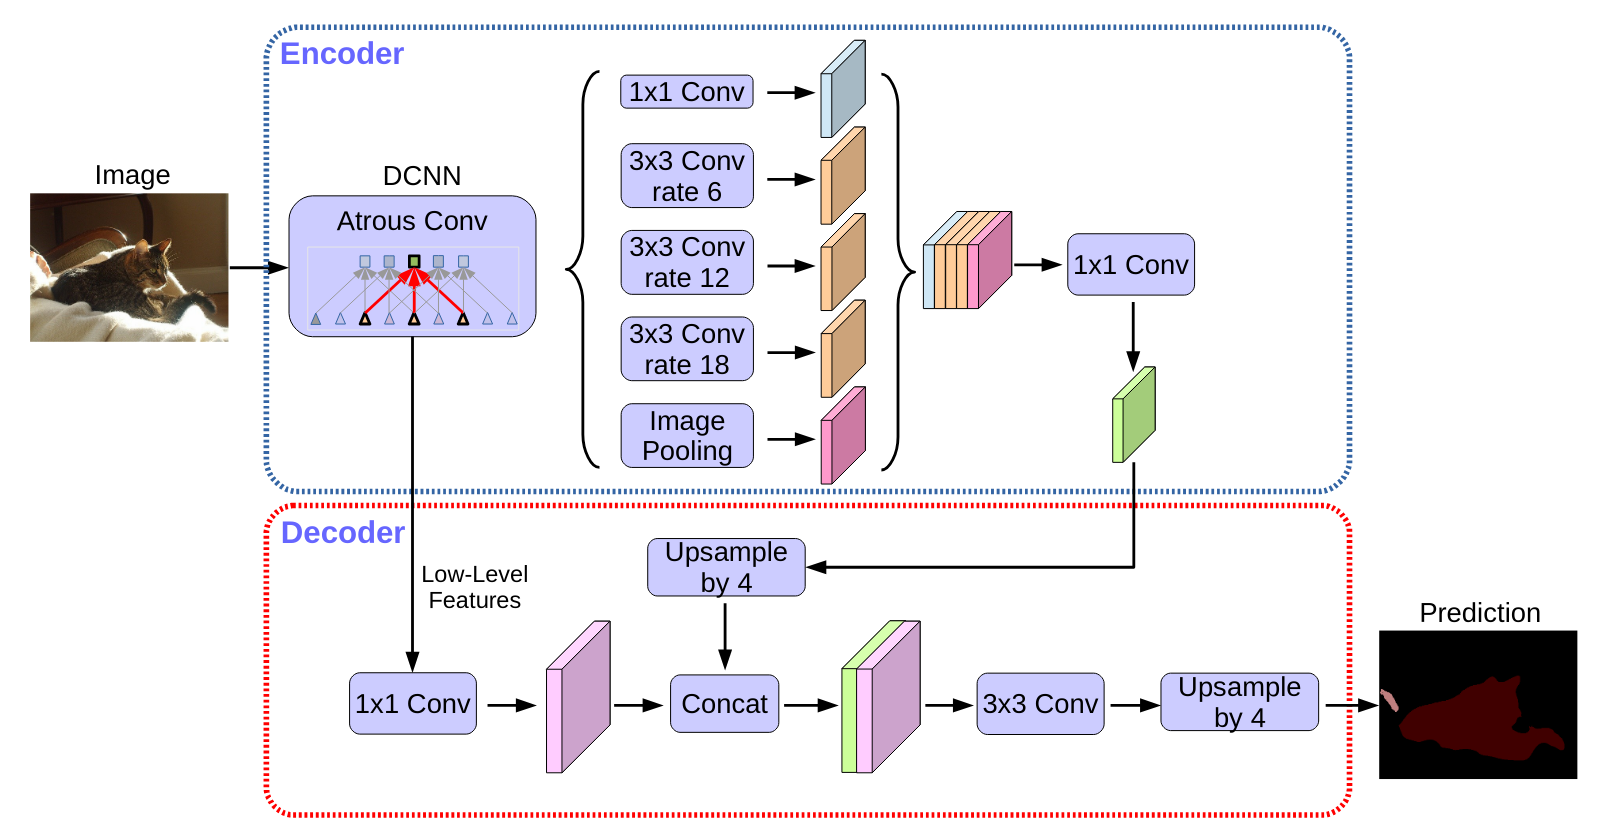
\includegraphics[width=.9\linewidth]{./deeplabv3p.png}
\caption{\label{fig:deeplabv3p}Illustration of the DeepLabv3+ for semantic segmentation. In contrast to the original architecture, we only use 2 Atrous layers (instead of \(3\)) with dilation rates \(2\) and \(4\). Figure taken from \cite{chen18}}
\end{figure}


\subsection{Optimization}
\label{sec:org86c88d6}

As loss function, we experiment on the widespread binary cross-entropy loss,
and further experiment with the Dice loss.

The latter addresses the fact that the cross-entropy loss is merely a ``proxy'' objective,
i.e. one is usually not interest in minimizing the metric, but rather
another metric that has a direct interpretation in computer vision (such as Dice-score,
or IoU).

In particular, we set the Dice-loss to:

\[
\mathcal{L}_{Dice}(\hat{y}, y) = 1 - \frac{2 \sum (\hat{y} \odot y) + s}{\sum y + \sum \hat{y} + s}
\]

where \(y\) and \(\hat{y}\) are the true and predicted probability tensors, respectively,
\(s\) is a smoothness coefficient that avoids unstability of gradients when
the denominator is small, and \(\odot\) is the element-wise multiplication operator.

\subsection{Training details and implementation}
\label{sec:org6330d84}

To optimize the parameters of our model, we follow the standard stochastic gradient descent
approach.
We split the provided dataset in a training, validation, and test set
that form \(60\%\), \(20\%\), and \(20\%\) of the full dataset, respectively.

At each epoch, we shuffle the training set and sample batches of size of \(12\).
We set the learning rate to \(10^-2\) and reduce to \(10^-3\) after \(15\) epochs.
We set the total number of epochs to \(20\) by observing the convergence of the loss
on the validation set.

Our model trains in \(\sim 14\) minutes on a 6-core/2.8GHz CPU.

Our algorithms are implemented in PyTorch, and the code is available at \url{https://github.com/lejeunel/blueortho\_hw}.

\section{Results}
\label{sec:org2e19306}

As evaluation metric, we select the Dice-score given by:
\[
D(\hat{y}, y) = \frac{2 \sum(\hat{y} \odot y)}{\sum y + \sum \hat{y}}
\]

Quantitative evaluations give a Dice-score of \(99.2\%\) for the BCE loss, and \(99.4\%\) for the
Dice loss.

Previews of our predictions are shown on Fig. \ref{fig:test_prev}.
While the variation in Dice-score seem minimal, the visual results show that in general
the background is cleaner and the foreground-background transitions are sharper
using the Dice-loss.

\begin{figure}[htbp]
\centering
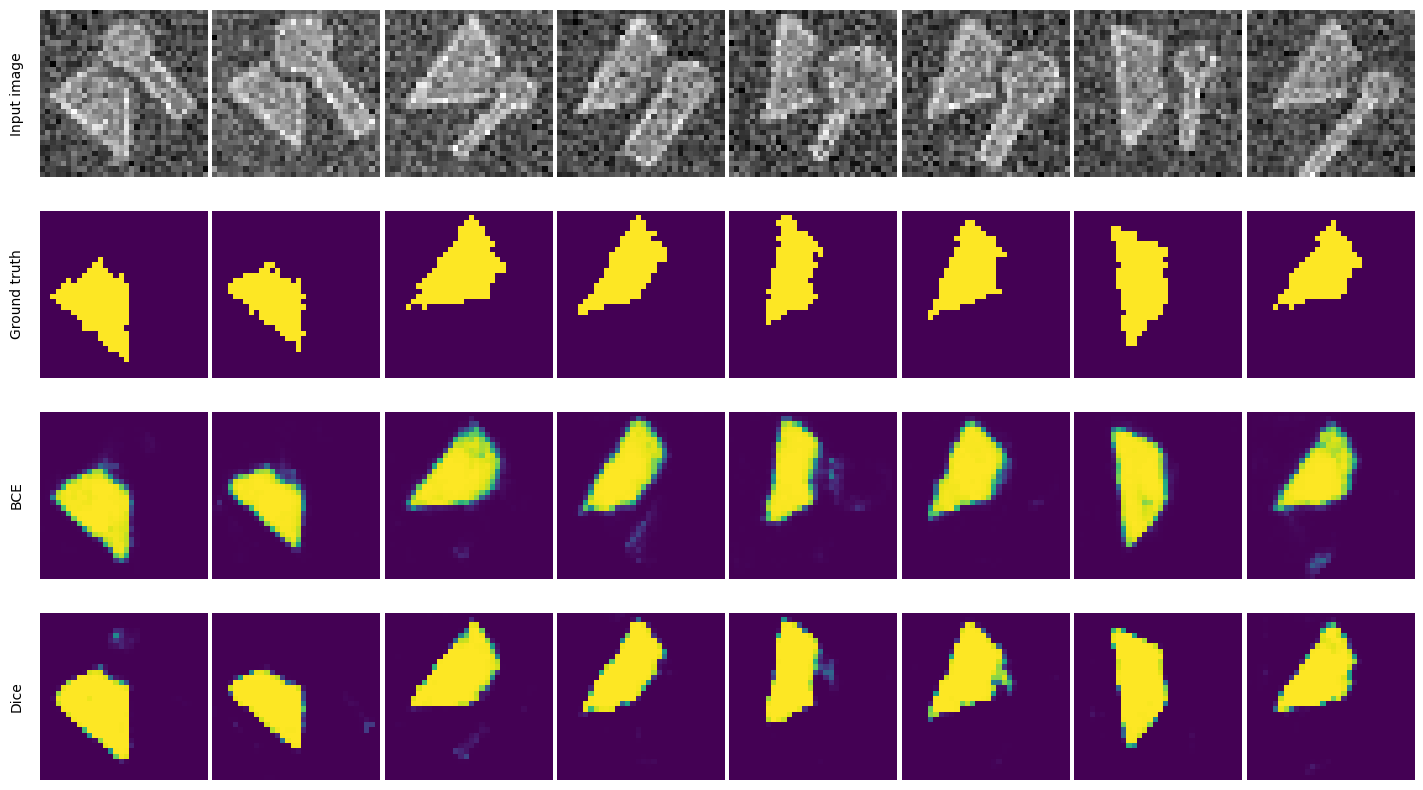
\includegraphics[width=.9\linewidth]{./test.png}
\caption{\label{fig:test_prev}Example predictions using the Binary Cross-Entropy loss (BCE), and the Dice loss.}
\end{figure}

\section{Conclusions}
\label{sec:orgfd0379a}

We proposed a simple Deep-Learning strategy to produce segmentation masks of synthetic
images of scapulae.
Our architecture proved to be both lightweight, computationally efficient and
provides good results.
In particular, we note that the Dice-loss is an interesting alternative to the
standard BCE-loss in this scenario. It is justified by the fact that it corresponds
to a metric that is directly interpretable, and produces visually sharper and cleaner predictions.

As potential improvements, one could explore the use of Atlases \cite{vakalopoulou18},
where one pre-defines a set of shapes that the network must adapt using deformation operators.
This might help to improve on the ambiguous cases where the scapulae and the humerus do
not show an obvious separation.


\printbibliography
\end{document}
